
% this file is called up by thesis.tex
% content in this file will be fed into the main document

%: ----------------------- introduction file header -----------------------
\chapter{State of the Art}\label{ch:soa}

\graphicspath{{soa/figures/}}

% -------------------------------------------------------------
% -- Related Work
% -------------------------------------------------------------

\section{Related Work}\label{sec:related-work}

In this chapter we analyze the current state of the art and limitations to facilitate the exploration of large and multilingual document collections. First, the tasks derived from processing the texts and enabling a semantic-aware exploration of the corpus are described. Then, an overview of the existing methods that perform these tasks is introduced. And finally, for each research area involved, the limitations that must be addressed to achieve the ultimate goal of facilitating documentary exploration are presented. The concepts that will be used throughout the rest of the thesis are here introduced. 

In order to browse large and multilingual document collections we need to process them in a way that is computationally affordable and provides enough knowledge to understand the relationships that arise. The annotation of human-readable documents is a well-known problem in the Artificial Intelligence (AI) domain in general and Information Retrieval (IR) and Natural Language Processing (NLP) fields in particular. Vector space models (VSM) \citep{Salton1983} were proposed to represent texts as vectors where each entry corresponds to a different term and the number at that entry corresponds to how many times that term is present in the text. The objective was twofold, on the one hand to make document collections manageable since we move from having lots of terms for each text to only one vector per document with defined dimension, and on the other hand to have representations based on metric spaces where calculations can be made, for example comparisons by measuring vector distances. The definition and number of dimensions for each vector are key aspects in a VSM. Traditional retrieval tasks over large collections of textual documents highly rely on individual features like term frequencies (TF) \citep{Hearst1999}. A representational space is created where each term in the vocabulary is projected by a separate and orthogonal dimension. All terms in a document are treated as equally descriptive. To overcome this problem, Term-Frequency Inverse-Document Frequency (TF-IDF) \citep{Manning2008} relativizes the relevance of each term with respect to the entire corpus. TF-IDF calculates the importance of a term for a document, based on the number of times the term appears in the document itself (term frequency - TF) and the number of documents in the corpus, which contain the term (document frequency - DF). The absence of semantic information and the notion of word sequences, and the high-number of dimensions are the main drawbacks of these approaches that lead to the emergence of other techniques. 

New ways of characterizing documents based on the automatic generation of models surfacing the main themes covered in the corpus are developed during recent years. Among them, text embedding proposes transforming texts into low-dimensional vectors by prediction methods based on (i) word sequences or (ii) bag-of-words. The first approach assumes words with similar meanings tend to occur in similar contexts. It considers word order relevant and is based on Neural Models (NM) that learn word vectors from pairs of target and context words, where context words are taken as words observed to surround a target word. Document vectors are usually created by taking the word vectors they contain or by considering them as target and context items. Skip-gram with negative sampling (Word2Vec) \citep{Mikolov2013c} and Global Vectors (GloVe) \citep{pennington2014} are indeed the most popular methods to learn word embeddings due to its training efficiency and robustness \citep{levy2015}. The second approach does not consider the order of the words to be relevant, but their frequency is. It assumes words with similar meanings will occur in similar documents. Topic models \citep{Deerwester1990, Hofmann2001, Blei2003} are the main methods based on this approach. This second approach is used in our work since \textit{we are not only interested in representing words and documents, but we also seek internal structures that can provide knowledge about the collection as a whole}.

Probabilistic Topic Models (PTM) \citep{Hofmann2001,Blei2003} are statistical methods based on bag-of-words that analyze the words of the original texts to discover the themes that run through them, how those themes are connected to each other, or how they change over time. PTM do not require any prior annotations or labeling of the documents. The topics emerge, as hidden structures, from the analysis of the original texts. These structures are topics distributions, per-resource topic distributions or per-resource per-word topic assignments. In turn, a topic is a distribution over terms that is biased around those words associated to a single theme. This interpretable hidden structure annotates each resource in the collection and these annotations can be used to perform deeper analysis about relationships between resources. Topic-based representations bring a lot of potential when applied over different IR tasks, as evidenced by recent works in different domains such as scholarly  \citep{Gatti2015}, health \citep{Lu2016, TapiNzali2017}, legal \citep{ONeill2017, Greene2016}, news \citep{He2017} and social networks \citep{Cheng2014a}. Topic modeling provides us an algorithmic solution to organize and annotate large collections of textual documents according to their topics.

The simplest generative topic model is \textit{Latent Dirichlet Allocation} (LDA) \citep{Blei2003}. Along with \textit{Latent Semantic Analysis} (LSA) \citep{Deerwester1990} and \textit{Probabilistic Latent Semantic Analysis} (pLSA) \citep{Hofmann2001} are part of the field known as topic modeling. They are well-known latent variable models for high dimensional data, such as the bag-of-words representation for textual data or any other count-based data representation. They try to capture the intuition that documents can exhibit multiple themes. Each document exhibits each topic in different proportion, and each word in each document is drawn from one of the topics, where the selected topic is chosen from the per-document distribution over topics. All the documents in a collection share the same set of topics, but each document exhibits these topics in a different proportion. Texts are described as a vector of counts with $W$ components, where $W$ is the number of words in the vocabulary. Each document in the corpus is modeled as a mixture over $K$ topics, and each topic $k$ is a distribution over the vocabulary of $W$ words. Formally, a topic is a multinomial distribution over words of a fixed vocabulary representing some concept. Depending on the function used to describe that distribution there are different algorithms to create topic models. While LSA and pLSA propose a singular value decomposition, LDA, influenced by the generative Bayesian framework to avoid some of the over-fitting issues that were observed with pLSA, suggests the use of a Dirichlet function. It is a continuous multivariate probability distribution parameterized by a vector of positive reals whose elements sum to 1.  It is continuous because the relative likelihood for a random variable to take on a given value is described by a probability density function, and is multivariate because it has a list of variables with unknown values. In fact, the Dirichlet distribution is the conjugate prior of the categorical distribution and multinomial distribution and is responsible for, unlike LSA and pLSA, LDA can infer topic distributions in texts that have not been used during training.

Topic models are not restrictive clustering models where each document is assigned to one cluster, but allows documents to exhibit multiple topics. The topics covered in a set of documents are discovered from the own corpus and feature vectors are topic distributions expressed as vector of probabilities. Taking into account this premise, the similarity between two topic-based resources is based on the distance between their topic distributions, which can be also seen as two probability mass functions. A commonly used metric is the \textit{Kullback-Liebler} (KL) divergence. However, it presents two major problems: (1) when a topic distribution is zero, KL divergence is not defined and (2) it is not symmetric, which does not fit well with semantic similarity measures that are usually symmetric \citep{Rus2013}.

\textit{Jensen-Shannon} (JS) divergence \citep{Rao1982,Lin1991} solves these problems considering the average of the distributions as below \citep{Celikyilmaz2010}:

\begin{equation}
JS(p,q) = \sum\limits_{i=1}^K p_{i}*\log \frac{2*p_{i}}{p_{i}+q_{i}}  +  \sum\limits_{i=1}^K q_{i}*\log \frac{2*q_{i}}{q_{i}+p_{i}}
\label{eq:jsdivergence}
\end{equation}
where  $K$ is the number of topics and $p,q$ are the topics distributions

It can be transformed into a similarity measure as follows \citep{Dagan1998} :

\begin{equation}
sim_{JS}(D_i , D_j) = 10^{- JS(p,q)}
\label{eq:simjs}
\end{equation}
where  $D_i,D_j$ are the documents and $p,q$ the topic distributions of each of them.


\textit{Hellinger} (He) distance is also symmetric and is used along with JS divergence in various fields where a comparison between two probability distributions is required \citep{Blei2007a,Hall2008,Boyd-Graber2010}:

\begin{equation}
	He(p, q) = \frac{1}{\sqrt{2}}\cdot\sqrt{\sum\limits_{i=1}^K (\sqrt{p_i} - \sqrt{q_i})^2)}
	\label{eq:hedistance}
\end{equation}

It can be transformed into a similarity measure by subtracting it from 1 \citep{Rus2013} such that a zero distance means max. similarity score and vice versa:

\begin{equation}
	sim_{He}(D_i, D_j) = 1 - He(p,q)
	\label{eq:simhe}
\end{equation}

However, all these metrics are not well-defined distance metrics, that is, they do not satisfy triangle inequality \citep{Charikar2002}. This inequality considers $d(x, z) <= d(x, y) + d(y, z)$ for a metric $d$ \citep{Griffiths2007} and places strong constraints on distance measures and on the locations of points in a space given a set of distances. As a metric axiom, the triangle inequality must be satisfied in order to take advantage of the inferences that can be deduced from it. Thus, if similarity is assumed to be a monotonically decreasing function of distance, this inequality avoids the calculation of all pairs of similarities by considering that if $x$ is similar to $y$ and $y$ is similar to $z$, then $x$ must be similar to $z$. 

\text{S2JSD} was introduced by \citep{Endres2003} to satisfy the triangle inequality. It is the square root of two times the $JS$ divergence:

%S2JSD formula
\begin{equation}
    S2JSD(P,Q) = \sqrt{2*JS(P,Q)}
\label{eq:s2jsd}
\end{equation}

\section{Research Areas}

This thesis aims to enable a semantic-aware exploration of the knowledge arising from large and multilingual document collections by exploiting the capabilities of topic models and their metric spaces. There are several research areas of ongoing related work. 

The first one is \textbf{topic creation and reuse}, key for understanding the steps needed to transform the unstructured data from a text into numerical values based on probabilistic topics. \textit{The way in which topic models are created and reused is crucial to addressing large-scale analysis}. 

The second area is \textbf{topic explainability}, which refers to the capacity of topics to capture and describe the content of a text. Topic explainability is important for \textit{making understandable the relationships that are derived from topic distributions}. 

The third area is \textbf{document similarity}, where the ability to measure the \textit{semantic difference between texts from the distance between their topic distributions is addressed}. 

Finally, the fourth area is \textbf{multilingual topics}, as we aim to explore collections of texts written in different languages through their topic-based relationships. A \textit{strategy to relate the topics of each language is needed}. 

These four areas are closely related to each other. Having efficient thematic representations of texts, distance metrics based on shared themes, and mechanisms to abstract the particularities of a language to represent the themes, may help to organize large multilingual document collections.

Each area and its limitations are described below. A summary can be found in Table~\ref{table:limitations}.

\begin{table}[!htbp]
\centering%
\begin{tabularx}{\linewidth}{bbb}
\toprule
\heading{Area} & \heading{Scope}& \heading{Limitation} \\
\midrule
\midrule
large-scale topic creation & process texts and train topic models from large corpora & no scalable frameworks that integrates both tasks  \\
\midrule
topic reuse & calculate distributions from existing topic models & no unified models for exchanging topic models \\
\midrule
topic explainability & describe and relate documents by topics & high dimensional models makes them difficult to interpret\\
\midrule
document similarity & compare topic distributions by measuring their distances & unaffordable complexity in large collections  \\
\midrule
multilingual topics & topic distributions across languages & parallel or comparable training data required\\
\bottomrule
\end{tabularx}
\caption{Research areas and limitations.}
\label{table:limitations}
\end{table}



\subsection{Topic Creation and Reuse}
\label{sec:topic-reuse}

Textual content usually includes non-relevant information and keeping only what can bring value for the involved agents (general consumers, experts, companies, investors...) becomes a challenge. A necessary first step before leveraging documents for knowledge-intensive tasks is to preprocess them following different techniques. Recent studies \citep{Westergaard2017} have shown that mining full-text articles gives consistently better results than only using sections or summaries. Given the size limitations and concise nature of summaries, they often omit descriptions or results that are considered to be less relevant but still are important for some IR tasks \citep{Divoli2012}.  Since this behavior is present in many other domains, our interest is focused on processing full texts, not only summaries or parts of texts, as we will show in the remainder of this thesis.

Exists a broad set of algorithms able to analyze text for producing annotations at very different levels of granularity: from minimal units such as terms and entities, to descriptors at the level of the entire collection such as  summaries or topics. Methods to perform Part-of-Speech (PoS) tagging,  Named Entity Recognition (NER) tasks, or topic modeling following the LDA or any other approach. But their implementations have been designed to work in an isolated, non-collaborative way \citep{Manning2014TheToolkit, Agerri2014}. They have not paid special attention to facilitating their interoperability and use closed formats to manage their data  which increase the technological dependence and limits their reuse and their expansion possibilities. For example, a topic model trained in Mallet\footnote{\url{http://mallet.cs.umass.edu}} can only make inferences if it is used from Mallet itself or using its libraries, since \textbf{\textit{there is no unified format for distributing topic models}} and each resource defines its own. In that example, the fact that Mallet is implemented in Java prevents reusing their models from Python or any other programming language. However, there are NLP tools (e.g. spaCy\footnote{\url{https://spacy.io}}) that have been provided through open services  decoupled from their technical development (e.g Explosion\footnote{\url{https://github.com/explosion/spacy-services}}).

Some approaches have advanced in this direction and offer the creation and exploitation of topic models through an API based on libraries\footnote{\url{https://bab2min.github.io/tomotopy}} or web services\footnote{\url{https://github.com/D2KLab/ToModAPI}}\citep{Lisena:NLPOSS2020}, but they are focused on the operations that can be performed on the model rather than abstracting the topic model as a resource. Others provide local\footnote{\url{https://onnx.ai/}} or remote\footnote{\url{https://vespa.ai}} ecosystems where create and reuse learning models, but their format is not open and cannot be used out of the environment. To the best of our knowledge, the efforts made do not propose a unified model to exchange topic models, understood as an already accepted standards-based format. In this thesis we propose \textit{reusable topic models and a scalable framework to create and use them}.  
 

\subsection{Topic Explainability}
\label{sec:topic-explainability}

Even though distance metrics mentioned in Section~\ref{sec:related-work} have been proposed and used in the SoA, making sense out of the similarity score based on compare topic distributions is not easy. As shown in figure \ref{fig:topic_distances}, given a set of pairs of documents, their similarity scores vary according to the number of topics. So the distances between the same pairs fluctuate from being more to less distant when changing the number of topics, and are hence difficult to use for relate semantically documents. In this conditions, which of those distances is better representing the underlying collection?
\begin{figure}
\begin{center}
\begin{adjustbox}{minipage=0.50\linewidth,frame=0pt 3pt}
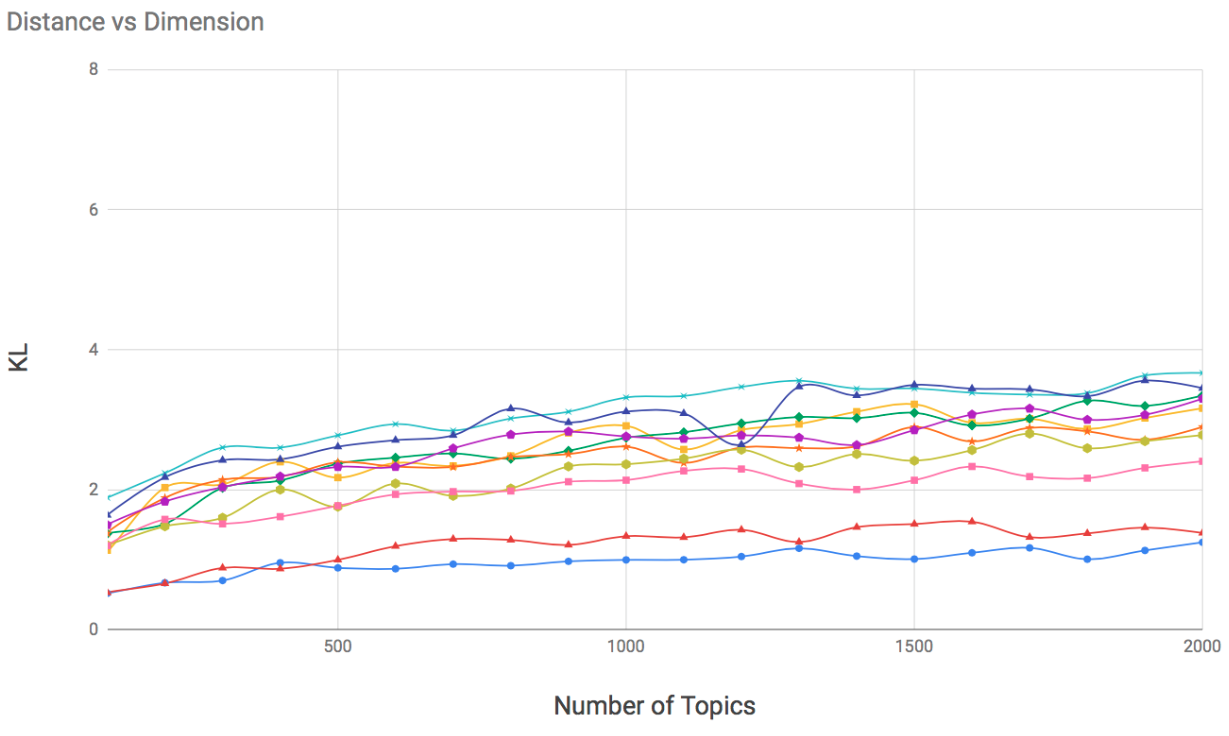
\includegraphics[width=\linewidth]{KL_100_2k.png}
\centering (a)
\end{adjustbox}
\hfill
\begin{adjustbox}{minipage=0.50\linewidth,frame=0pt 3pt}
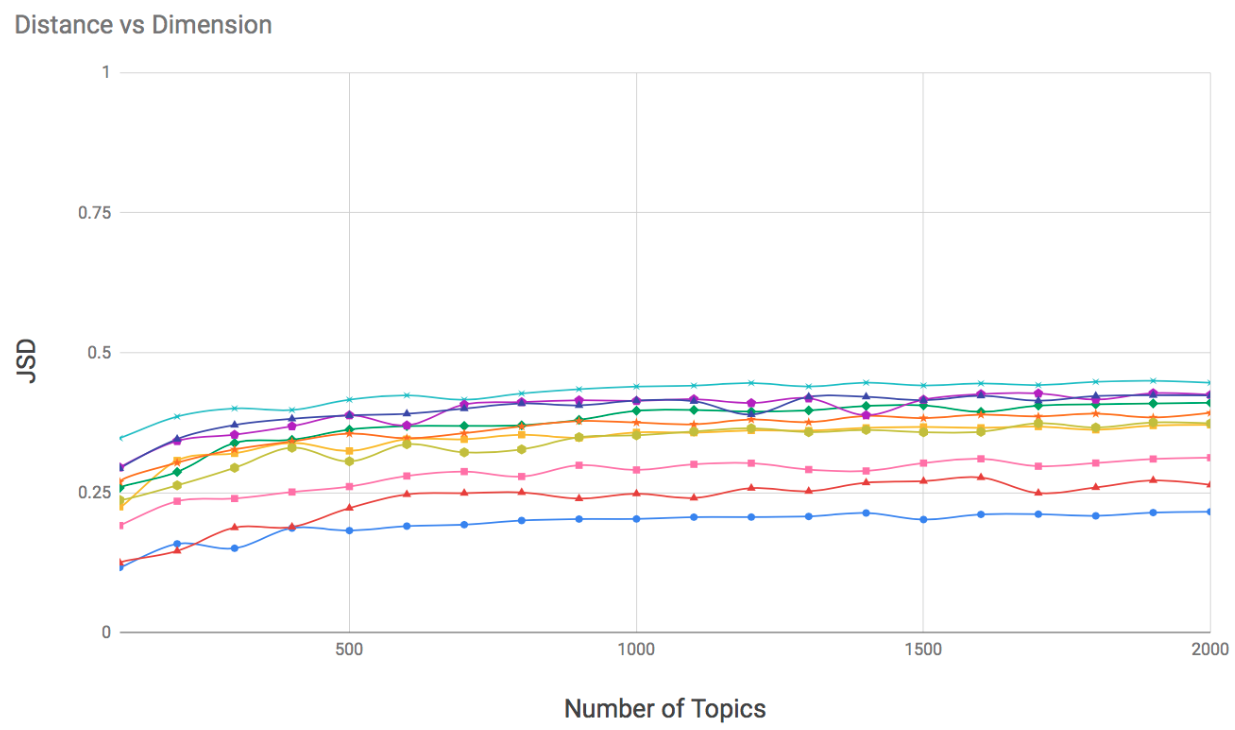
\includegraphics[width=\linewidth]{JSD_100_2k.png}
\centering (b)
\end{adjustbox}
\hfill
\begin{adjustbox}{minipage=0.50\linewidth,frame=0pt 3pt}
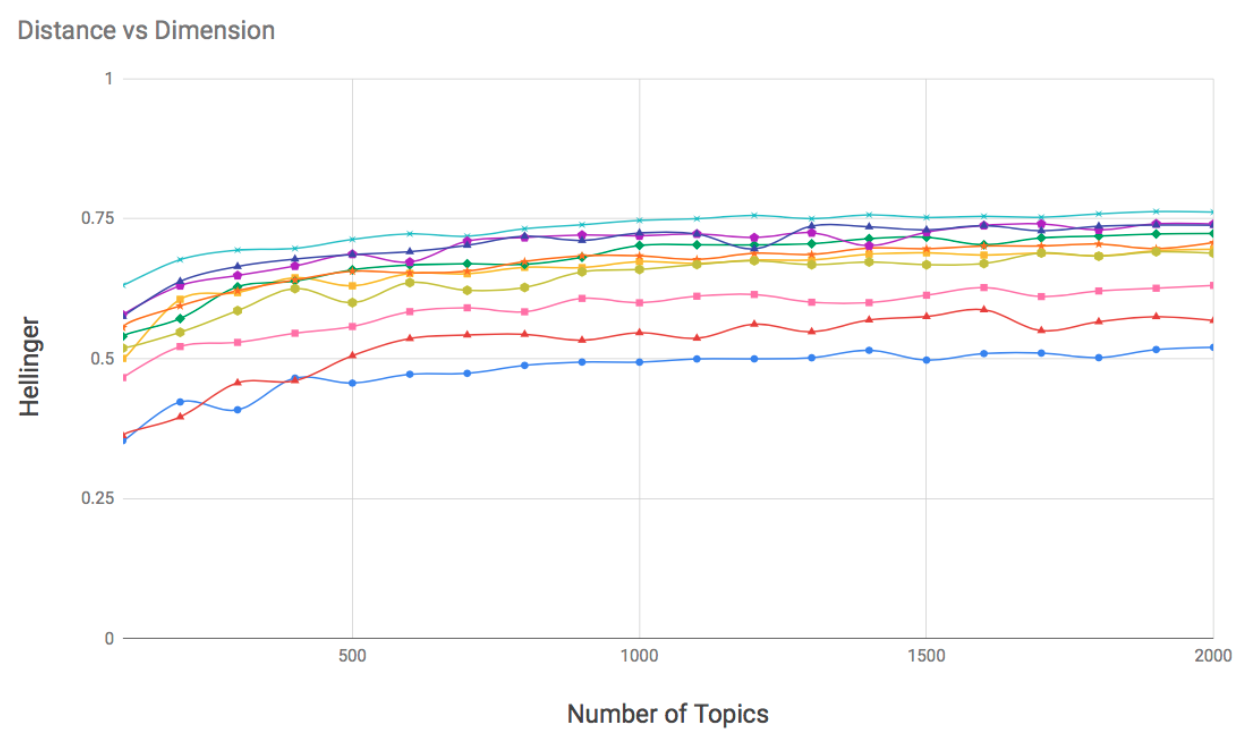
\includegraphics[width=\linewidth]{He_100_2k.png}
\centering (c)
\end{adjustbox}
\hfill
\begin{adjustbox}{minipage=0.50\linewidth,frame=0pt 3pt}
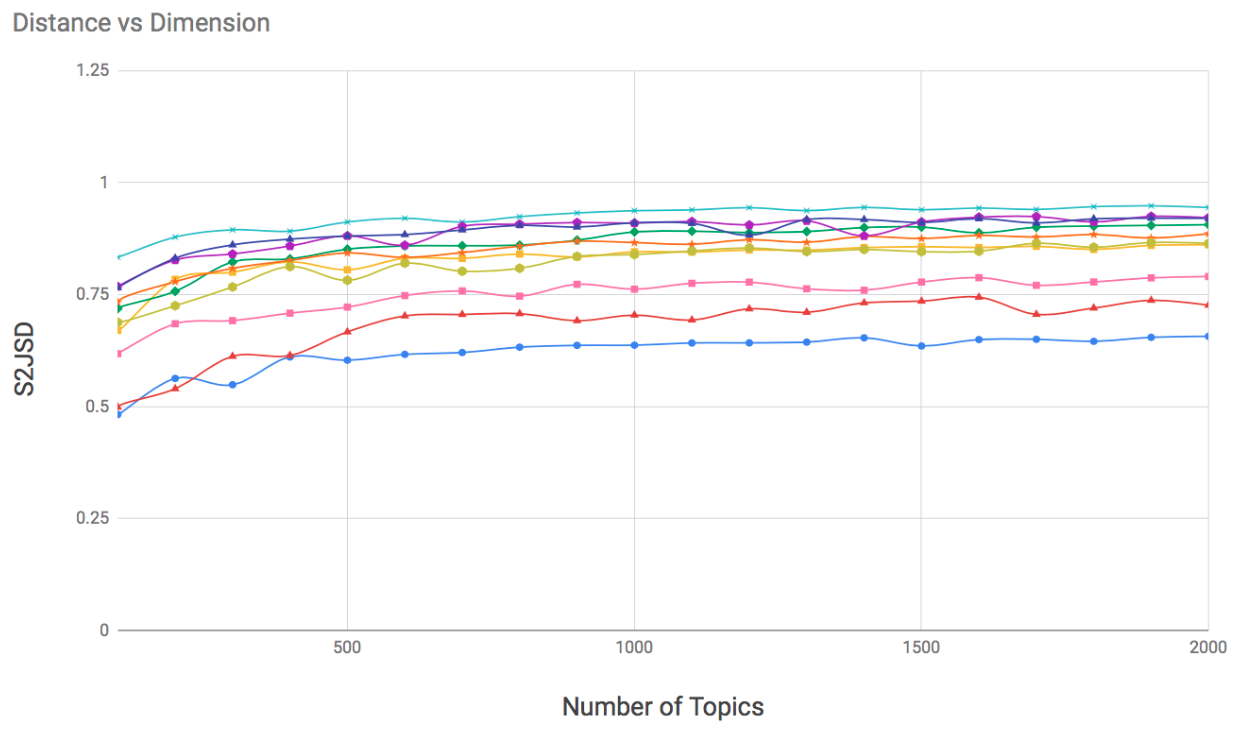
\includegraphics[width=\linewidth]{S2JSD_100_2k.png}
\centering (d)
\end{adjustbox}
\end{center}
\caption{Distance values of 10 pairs of documents calculated in topic models with 100-to-2000 dimensions. The Kullback-Liebler(a), Jensen-Shannon Divergence(b), Hellinger(c) and S2JSD(c) metrics are considered.}
\label{fig:topic_distances}
\end{figure}

Distances between documents based on topic distributions, because it is a vector space, generally increase as the number of dimensions of the space increases. This is due to the fact that as the number of topics describing the model increases, the more specific the topics will be. Topics shared by a pair of documents can be broken down into more specific topics that are not shared by those documents. \textit{Document similarity is then dependent on the model used to represent documents when considering this type of metrics}. 

Each topic is drawn from a Dirichlet distribution with parameter $\beta$, while each document's mixture is sampled from a Dirichlet distribution with parameter $\alpha$. These two priors, $\alpha$ and $\beta$, are also known as hyper-parameters of a topic model and they set the probability that a document or a word, respectively, contains more than one topic. We know that absolute distances between documents vary when we tune those hyper-parameters differently, but we also see that ``relative distances" also change. Imagine that we have two documents, A and B, and one topic model, M1. The distance from the topic distribution of A to B is less than from A to C. However, in a second topic model, M2, trained with the same documents as M1 but with different hyper-parameters, the distance from the topic distribution of A to C is less than to B (cross-lines in fig \ref{fig:topic_distances}). This behaviour highlights the \textbf{\textit{difficulty of establishing absolute similarity thresholds and the complexity to measure distances taking into account all dimensions}}. If we consider that documents are similar when their distance is lower than 0.2, a pair of documents may be similar when they are represented in low-dimensional topic models, and not similar when high-dimensional models are used to represent them. Distance thresholds should be model-dependent rather than general and metrics flexible enough to handle dimensional changes. In this thesis we have gone beyond the thematic and low-dimensional feature space created by topic models and propose a \textit{ hierarchical feature space suitable for big real-world data sets, where documents are only described by their most relevant topics}.


\subsection{Document Similarity}

In addition, document similarity comparisons are too costly to be performed in huge collections of data and require more efficient approaches than having to calculate all pairwise similarities. Using a naive approach creating a similarity matrix with all document comparisons takes $O(n^2)$ time (where $n$ is the number of documents), so obtaining all possible pairs of similarities in a large collection of documents (e.g. a corpus of 32 million patents) can be unfeasible because of the exponential cost of comparing every pair of elements. Many different approaches have been proposed to reduce this complexity. For instance, computation can be approximated by a nearest neighbors (ANN) search problem \citep{Indyk1998}. ANN search is an optimization problem that finds nearest neighbors of a given query in a metric space of $n$ points. 

Due to the low storage cost and fast retrieval speed, hashing is one of the most popular solutions for ANN search \citep{Zhen2016}. This technique transforms data points from the original feature space into a binary-code space, so that similar data points have larger probability of collision (i.e. having the same hash code). This type of formulation for the document similarity comparison problem has proven to yield good results in the metric space \citep{Krstovski2011} due to the fact that ANN search has been designed to handle distance metrics (e.g. cosine, Euclidean, Manhattan). But distance metrics between topic distributions should be information-theoretically motivated metrics ( e.g. Hellinger, Kullback-Leibler divergence, Jensen-Shannon divergence) since they compare density functions. 

These challenges can be tackled by hashing methods based on clusters of topics to measure similarity, instead of directly using their weights. Hashing methods transform the data points from the original feature space into a binary-code Hamming space, where the similarities in the original space are preserved. They can learn hash functions (data-dependent) or use projections (data-independent) from the training data \citep{Wang2016}. Data-independent methods, unlike data-dependent ones do not need to be re-calculated when data changes, i.e. adding or removing documents to the collection. Taking large-scale scenarios into account (e.g. Document clustering, Content-based Recommendation, Duplicate Detection), data independency is a key feature along with the ability to infer hash codes individually (for each document) rather than on a set of documents. Data-independent hashing methods depend on two key elements: (1) data type and (2) distance metric. For vector-type data, as introduced in section \ref{sec:related-work}, based on $l_p$ distance with $p \epsilon [0,2)$ lots of hashing methods have been proposed, such as p-stable Locality-Sensitive Hashing (LSH) \citep{Datar2004}, Leech lattice LSH \citep{Andoni2006}, Spherical LSH \citep{Terasawa2007}, and Beyond LSH \citep{Andoni2014}. Based on the $\theta$ distance many methods have been developed such as Kernel LSH \citep{Kulis2012} and Hyperplane hashing \cite{Vijayanarasimhan2014}. But only few methods handle density metrics in a simplex space, where topic distributions are projected. A first approach transformed the $He$ divergence into an Euclidean distance so that existing ANN techniques, such as LSH and k-d tree, could be applied \cite{Krstovski2013a}. But this solution does not consider the special attributions of probability distributions, such as Non-negative and Sum-equal-one. Recently, a hashing schema \citep{Mao2017} has been proposed taking into account the symmetry, non-negativity and triangle inequality features of the S2JSD metric for probability distributions. For set-type data, Jaccard Coefficient is the main metric used. Some examples are K-min Sketch \citep{Li2012}, Min-max hash \citep{Ji2013}, B-bit minwise hashing \citep{Li2010b} and Sim-min-hash \citep{Zhao2013}.

All of them have demonstrated efficiency in the search for similar documents, but none of them considers the search for documents (1) by thematic areas or (2) by similarity levels, nor they offer (3) an \textbf{\textit{explanation about the similarity obtained beyond the vectors used to calculate it}}. In addition, binary-hash codes drop a very precious information: the topic relevance. This thesis proposes a \textit{hash function-based approach that allows efficiently searching for related documents while maintaining topic-based annotation, preserving notion why two documents are related}.


\subsection{Multilingual Topic Alignment}

When the IR task is also cross-language, document retrieval must be independent of the language of the user's query. At execution time, the query in the source language is typically translated into a target language with the help of a dictionary or a machine-translation system. But for many languages we may not have access to translation dictionaries or a full translation system, or they can be expensive to execute, or expensive to train (lot of data required) in an online search system. In such situations it is useful to rely on smaller annotation units derived from the text so the full content does not need to be translated, for instance by finding correspondences with regard to the topics discussed in both the query and the documents being searched.

Some methods uses document-aligned corpora, where documents are grouped and constrained to the same topic distribution during training to align the different languages \citep{Smet2009, mimno-etal-2009-polylingual, Ni2009, Fukumasu2012, Zhang2013}, or theme-aligned corpora, where similar themes and ideas appear in all languages\citep{Graber2009}. Multilingual Probabilistic Topic Models (MuPTM) \citep{Vulic2015} have emerged in this area as a group of language-independent generative machine learning models that can be used on theme-aligned multilingual texts. They are based on LDA, adding supervised associations between languages by using \textit{parallel} corpora, with sentence-aligned documents (e.g. Europarl\footnote{https://ec.europa.eu/jrc/en/language-technologies/dcep} corpus), or \textit{comparable} comparable, with theme-aligned documents (e.g. Wikipedia\footnote{https://www.wikipedia.org/} articles), in multiple languages. Once a MuPTM has been generated, documents can be represented by data points in a single feature space based on topics to detect similarities among them exploiting inference results and using distance metrics. Due to its generic language-independent nature and the power of inference on unseen documents, MuPTM's have found many interesting applications in many different cross-lingual tasks. They have been used on cross-lingual event clustering \citep{DeSmet2009}, document classification \citep{10.1007/978-3-642-20841-6_45, Ni:2011:CLT:1935826.1935887},  semantic similarity of words \citep{Mimno:2009:PTM:1699571.1699627, Vulic:2012:DHC:2380816.2380872}, information retrieval \citep{10.1007/978-3-642-36973-5_9, ganguly-etal-2012-cross}, document matching \citep{Platt:2010:TDR:1870658.1870683, zhu-etal-2013-building}, and others. 

Other methods are based on word alignments from bilingual dictionaries instead of aligned corpora. Topic models emerge as distributions over crosslingual equivalence classes of words \citep{Jagarlamudi2010, zhang-etal-2010-cross, hao-paul-2018-learning}. A recent approach is placed between word and document alignments. It proposes crosslingual topic models using the language-independent categories assigned to each wikipedia article\citep{2020arXiv200911207P}. Instead of using bags-of-words to represent texts, which would be language dependent, it explores the references of each article and represents them through bags-of-links, using the categories of each reference to represent the texts.

In short, \textbf{\textit{the requirement of parallel/comparable corpora or dictionaries limits the usage of these models in many situations}}. There are not many document collections that can be used for training since large parallel corpora are rare in most of the use cases, especially for languages with fewer resources. Moreover, in order to incorporate new languages or update the existing associations, these models must be re-trained with documents from all languages at the same time, making it difficult to scale to large corpora \citep{Hao2018, Moritz2017}. We take MuPTM a step further by making it cross-lingual through representations based on topic hierarchies. Documents from multi-language corpora are described by expressions of language independent concepts and can then be efficiently browsed and related with other languages without the need for translation or parallel or comparable corpora. In this thesis we propose to \textit{automatically infer cross-lingual topics to browse multi-lingual document collections without the need for parallel or comparable corpus}. 
